\section{Introduction}\label{introduction}

\begin{frame}{Women Contribute Online Less Than Men}

\begin{itemize}[<+->]
\tightlist
\item
  Only 13\% women contributors on Wikipedia
\item
  Wikipedia entries about women are less likely to be complete
\item
  Only 5\% women contributors on StackOverflow
\item
  Less than 5\% women taking part in programming competitions (despite
  30\% in CS schools)
\end{itemize}

\end{frame}

\begin{frame}{Implications for individuals, firms \& society}

\begin{itemize}[<+->]
\tightlist
\item
  Narrow participation \(\leadsto\) lower profits
\item
  Less diversity \& creativity for innovation
\item
  Labor market discrimination
\item
  Platform content may reflect biased views
\end{itemize}

\end{frame}

\begin{frame}{A theory of gender imbalance}

We conjecture:

\begin{itemize}[<+->]
\tightlist
\item
  \textbf{Gamification} \& Incentives (e.g., competition, points,
  rankings)
\item
  Gender differences in \textbf{preferences} (e.g., risk aversion,
  competitive inclination)
\end{itemize}

Mechanisms under investigation

\begin{enumerate}
\def\labelenumi{\arabic{enumi}.}
\tightlist
\item
  Perceived gender composition in a competitive environment
\item
  \color{gray}{Collaboration incentives under gender imbalance [next study]}
\end{enumerate}

\end{frame}

\begin{frame}{Bayesian updating}

\begin{figure}
\centering
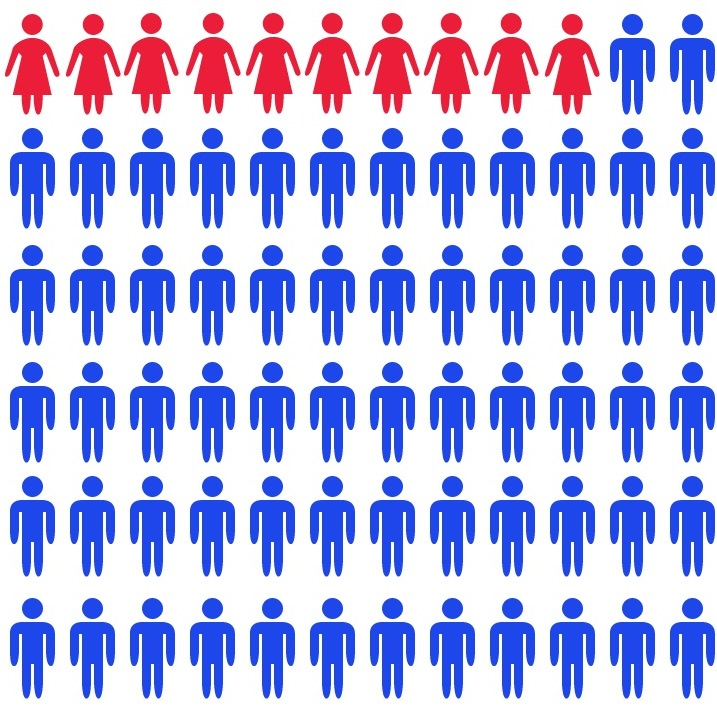
\includegraphics{female_fuel_for_the_digital_economy.jpg}
\caption{What are the odds of winning for gender XY?}
\end{figure}

\end{frame}

\begin{frame}{Role model}

\begin{figure}
\centering
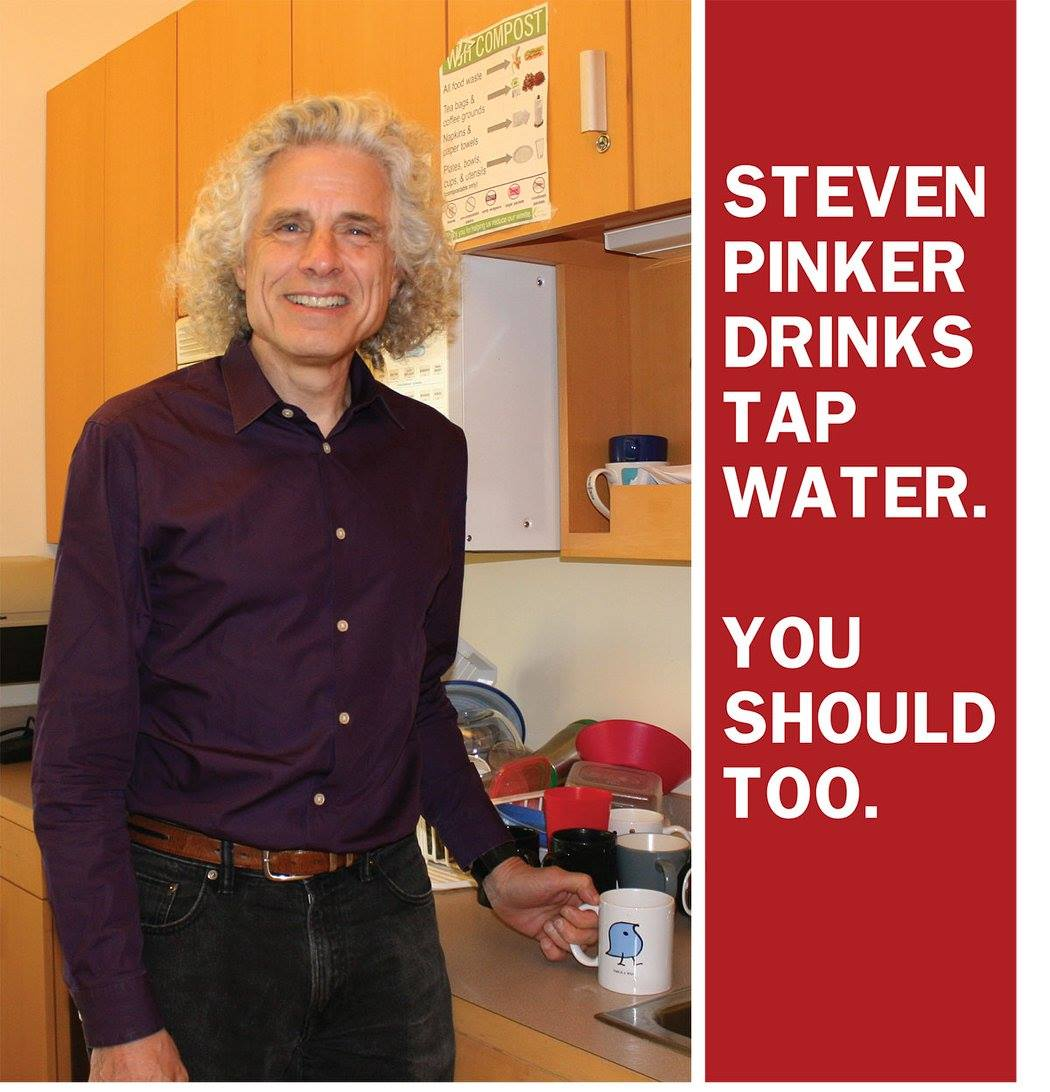
\includegraphics[width=0.5\textwidth]{tap_water_pinker.jpg}
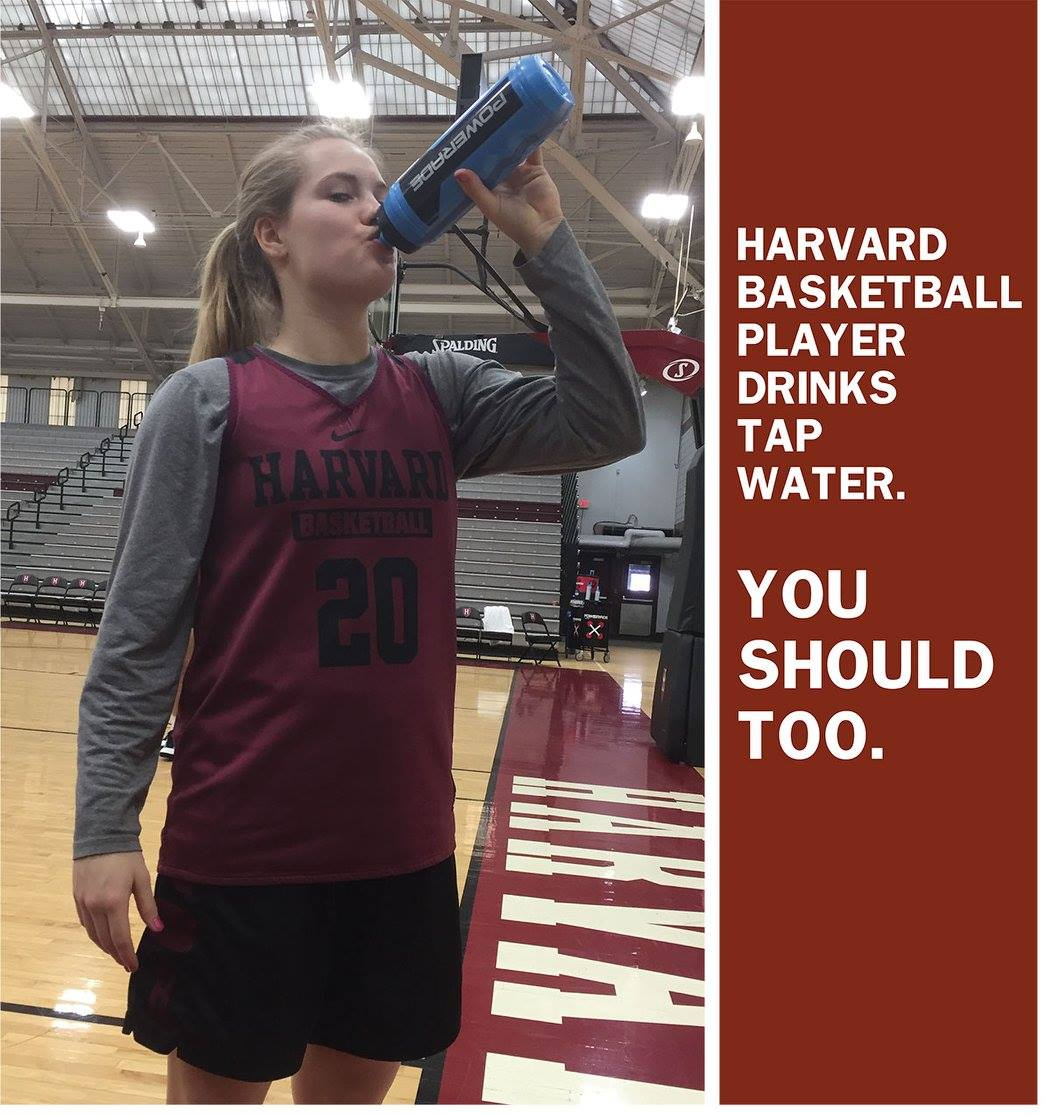
\includegraphics[width=0.5\textwidth]{tap_water_basket.jpg}
\caption{do I want to be successful in this?}
\end{figure}

\end{frame}

\begin{frame}

\begin{figure}
\centering
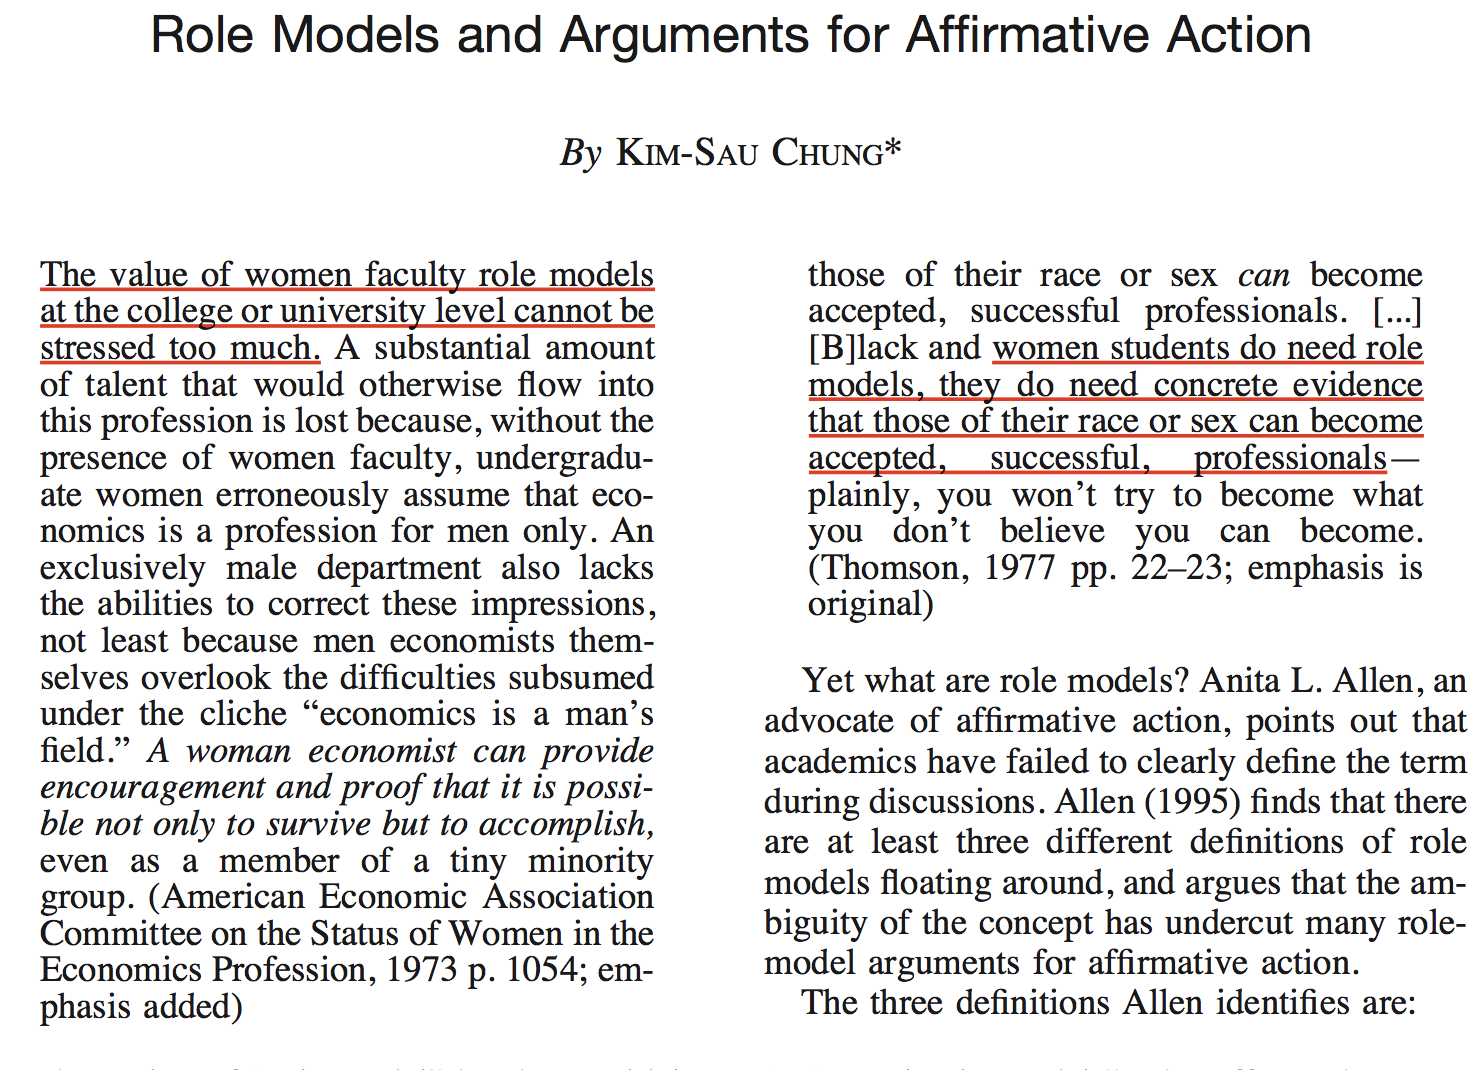
\includegraphics{aer-citation.png}
\caption{American Economic Review, 2000}
\end{figure}

\end{frame}

\section{Context and Data (HeroX.com)}\label{context-and-data-herox.com}

\begin{frame}{Gender participation in Herox.com}

The sex ratio is:

\begin{itemize}
\tightlist
\item
  2 men registrants for each woman (33 percent women)
\item
  2 men contributing for each woman (33 percent women)
\end{itemize}

\end{frame}

\begin{frame}

\begin{figure}
\centering
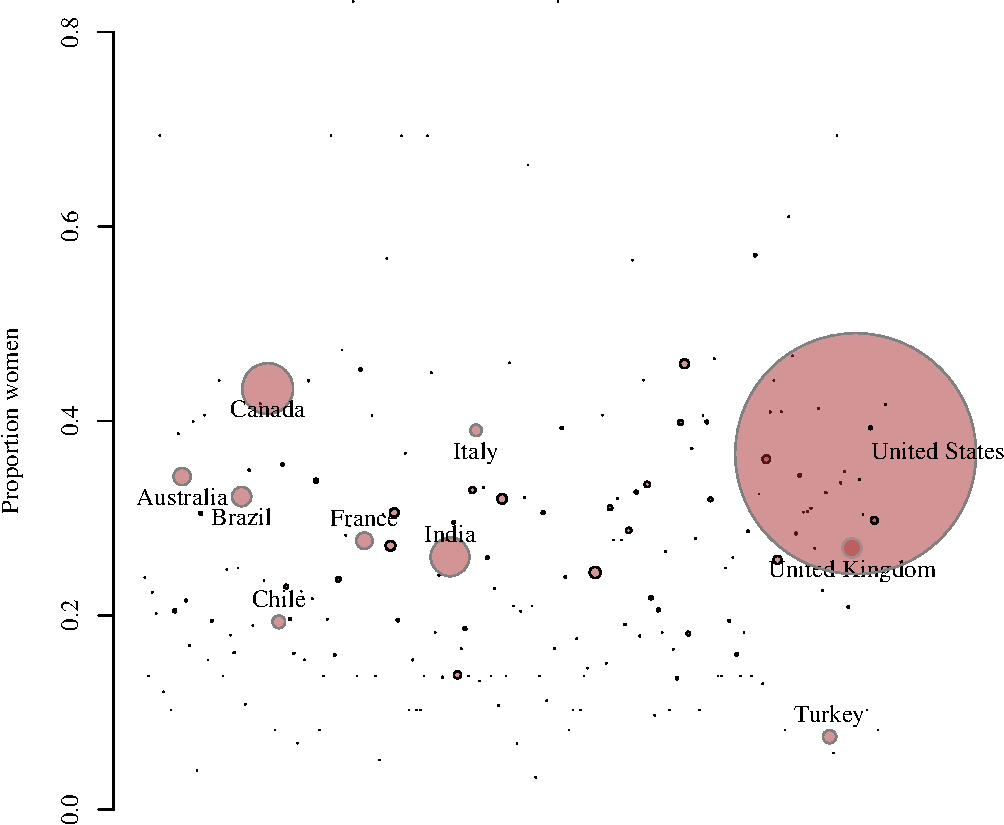
\includegraphics{Figures/bayes-1.pdf}
\caption{Proportion of women members by country}
\end{figure}

\end{frame}

\begin{frame}

\begin{figure}
\centering
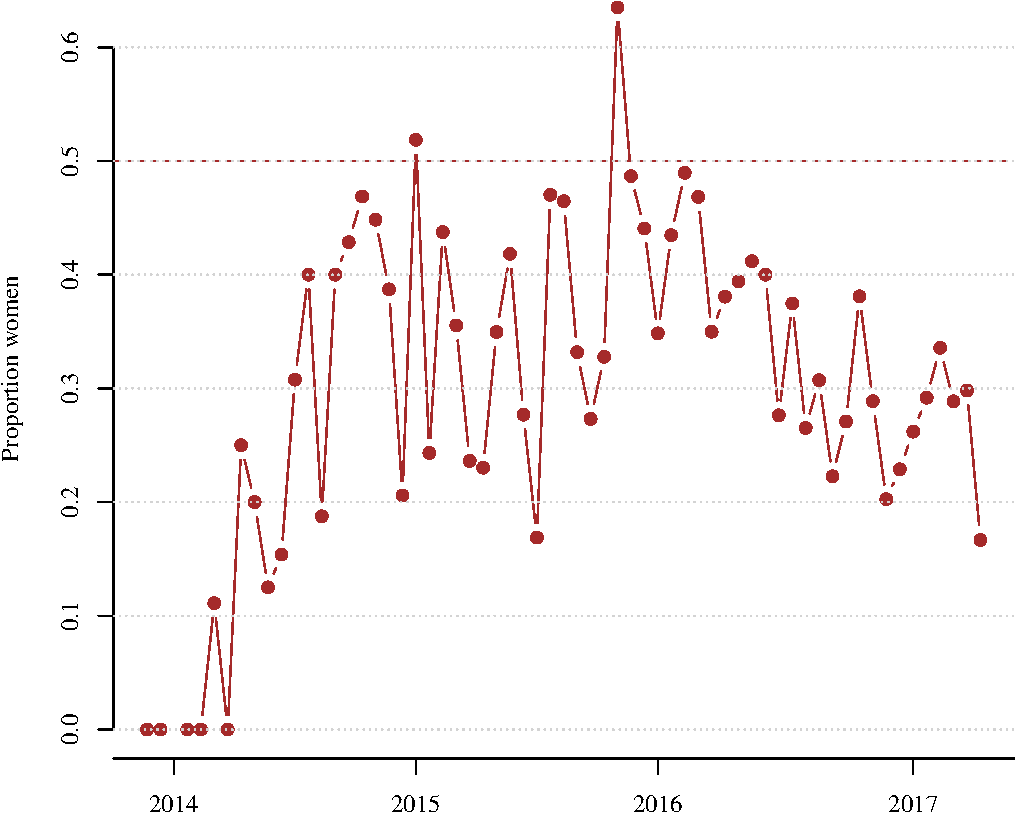
\includegraphics{Figures/overtime-1.pdf}
\caption{Proportion of women new members over time}
\end{figure}

\end{frame}

\begin{frame}

\begin{figure}
\centering
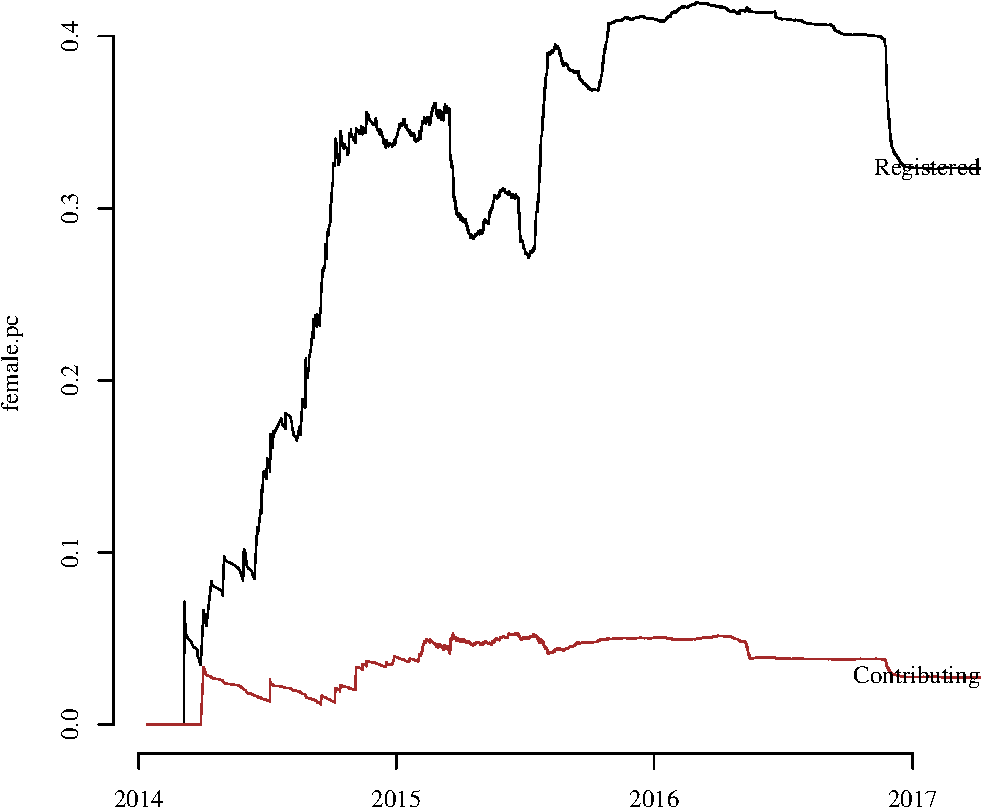
\includegraphics{Figures/cumsum-1.pdf}
\caption{Cumulative proportion of women over time}
\end{figure}

\end{frame}

\section{Experimental design}\label{experimental-design}

\begin{frame}{Winning members as ``Role models''}

\begin{figure}
\centering
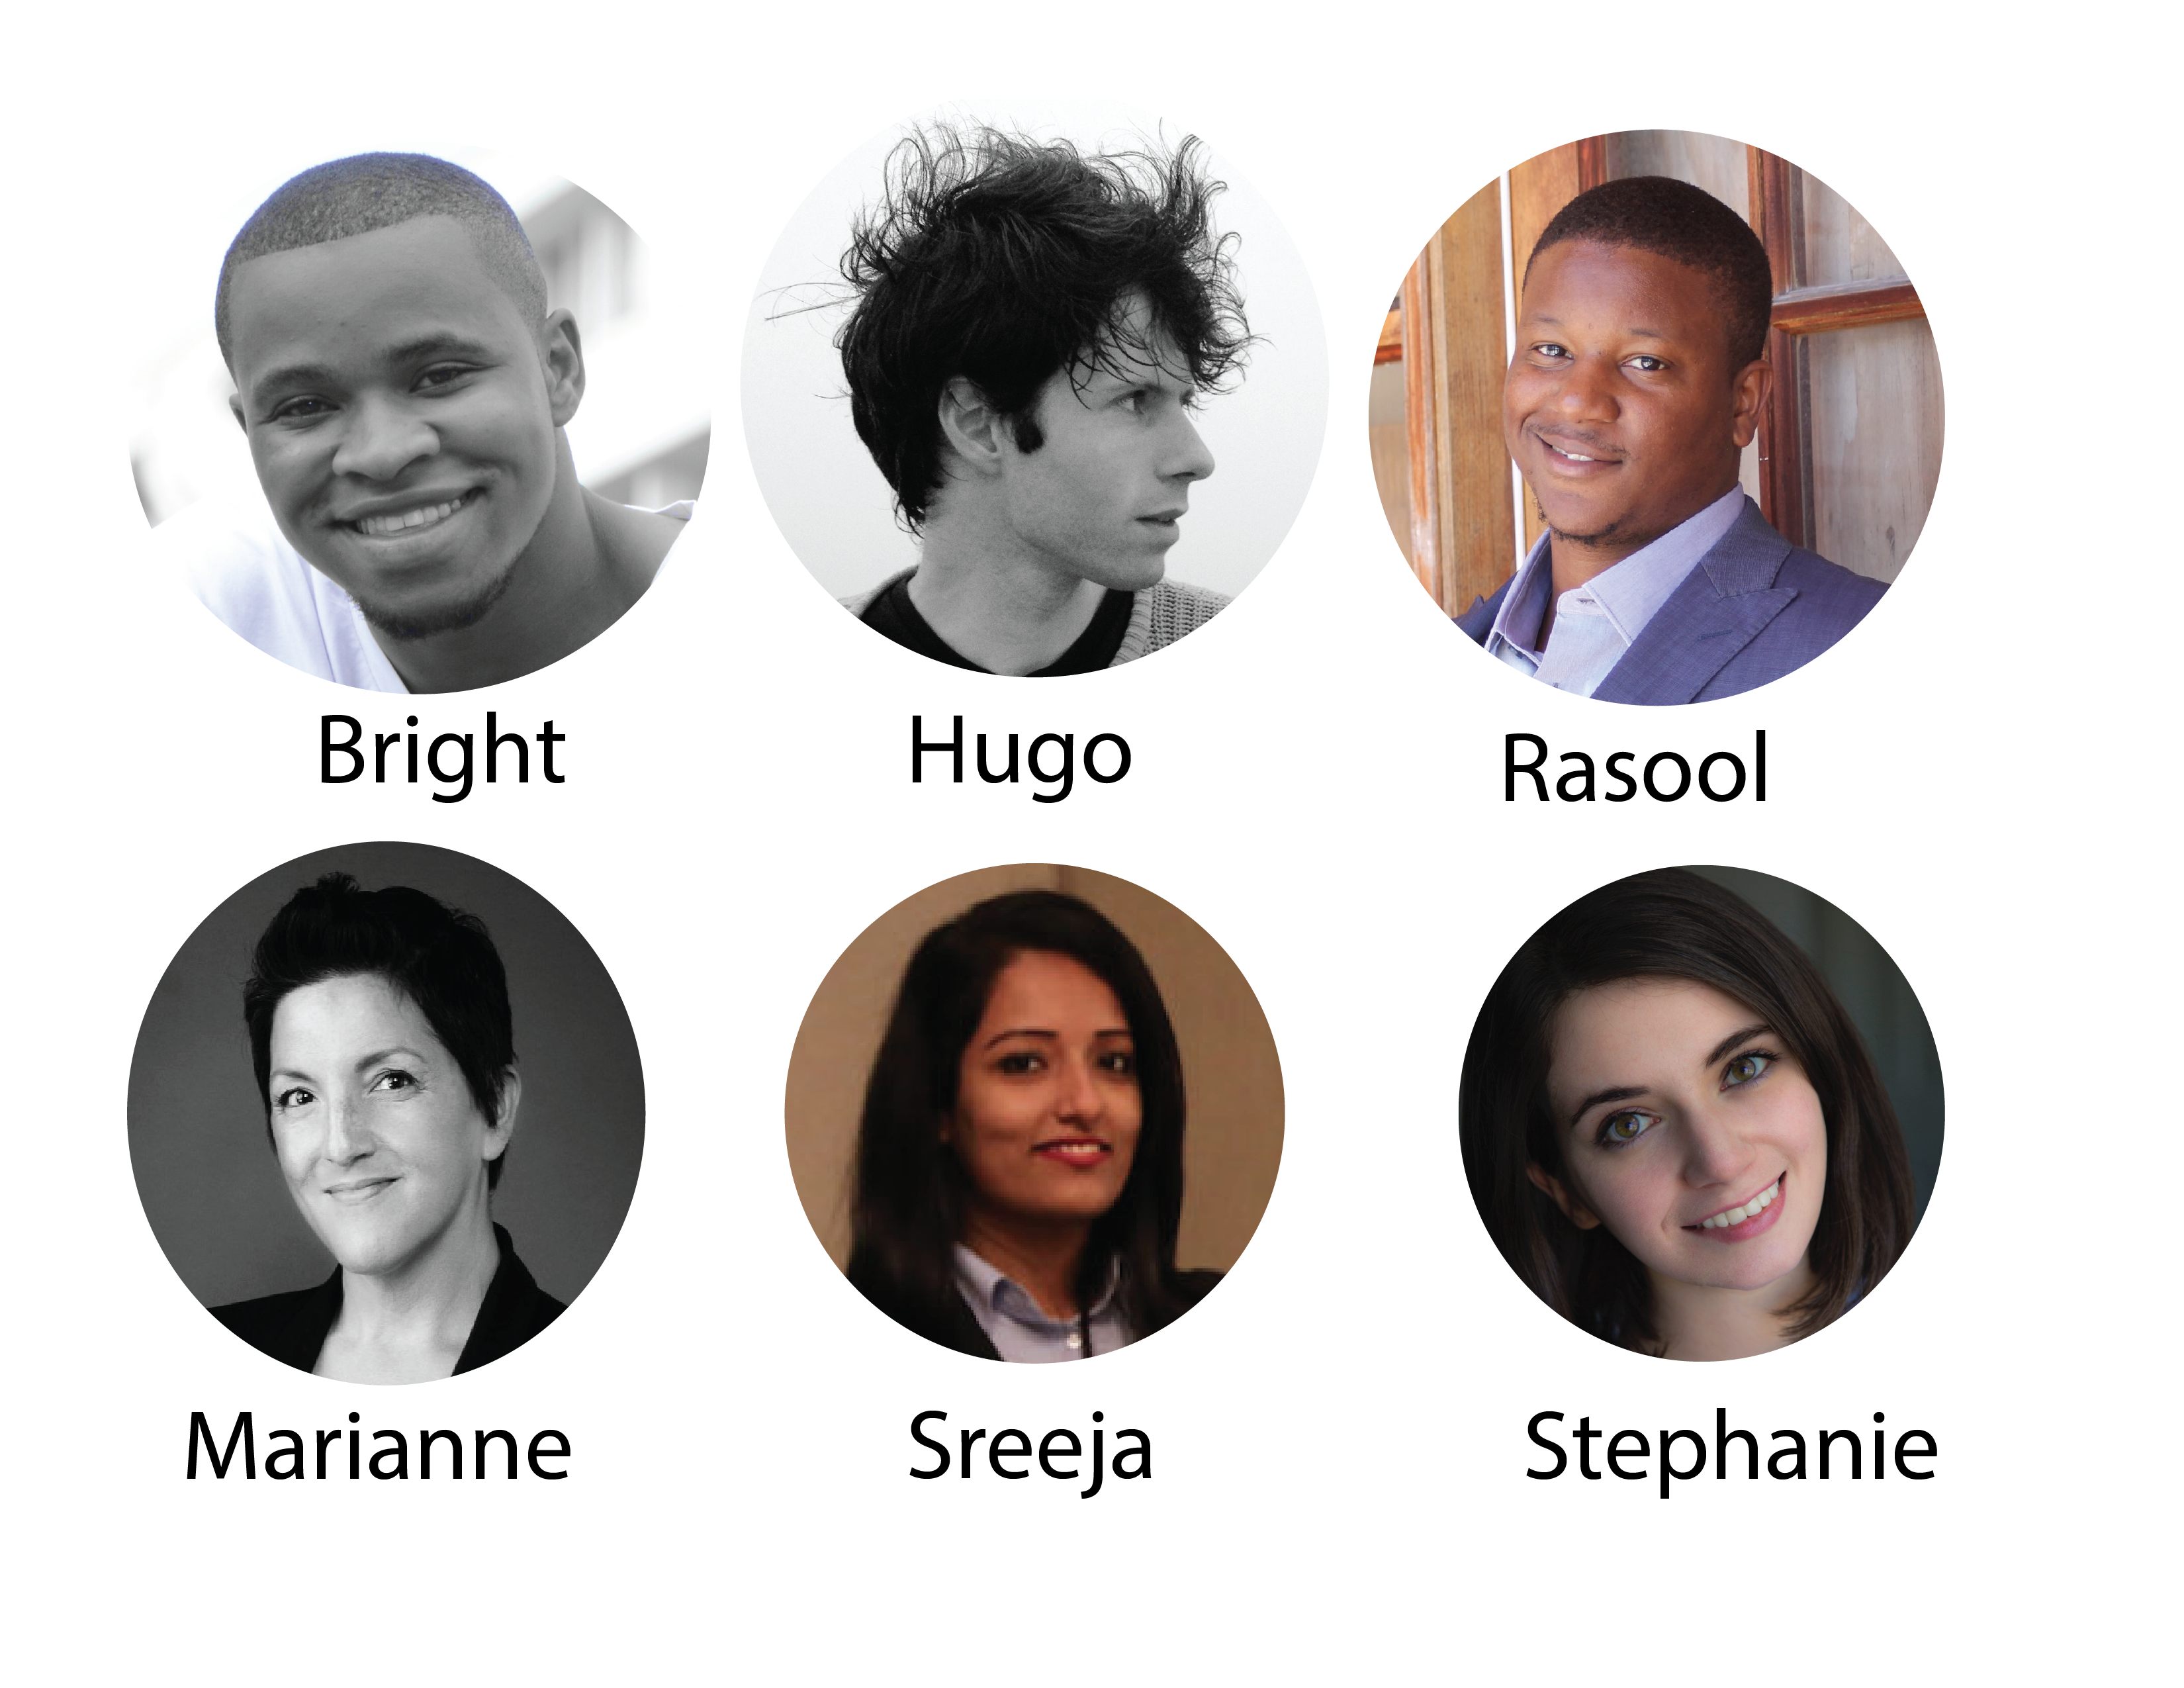
\includegraphics{herox_headshots-01.png}
\caption{Example of 6 recruited members}
\end{figure}

\end{frame}

\begin{frame}{Randomized intervention}

Send solicitation with \(k\) role models to \(60K\) HeroX members

\[
    \text{possible combinations} = \binom{m + f}{k} 
\]

\begin{block}{Example (\(k=2\), \(m=8\) and \(f=8\))}

\(16! / (14! 2!) = 16 * 15 / 2 = 120\) possible combinations
\(\leadsto\) \(60000/120=500\) subjects per combination

\end{block}

\begin{block}{Example (\(k=3\) \(m=6\) and \(f=6\))}

\(12! / (9! * 3!) = 12 * 11 * 10 / 6 = 220\) possible combinations
\(\leadsto\) \(\approx 270\) subjects per combination.

\end{block}

\end{frame}

\begin{frame}{How to pick \(m\), \(f\), and \(k\)?}

\begin{itemize}
\item
  Recruited 19 profiles (11 men and 8 women)
\item
  Examined and scored each profile according to:

  \begin{itemize}
  \tightlist
  \item
    Physical attractiveness
  \item
    Perceived age
  \item
    Perceived ethnicity
  \item
    ``Role model''
  \end{itemize}
\item
  Select \(f\) and \(m\) such that scores are balanced
\item
  Select \(k\) that gives high power
\end{itemize}

\end{frame}

\begin{frame}{The problem of causality}

\begin{block}{What we identify?}

\begin{itemize}
\item
  ``Causal effects'' for (1) individuals \& (2) profile combinations
\item
  Further assumptions needed for \textbf{interactions} (e.g., same
  gender, ethnicity) and \textbf{gender composition} {[}best we can do
  without ``lying''{]}
\end{itemize}

\end{block}

\begin{block}{Which ``causal effects''?}

\begin{itemize}
\item
  Intention-To-Treat (ITT) which ignores anything that happens after
  randomization.
\item
  Complier Average Causal Effect (CACE) which considers the effect on
  those who comply (i.e., who open their emails)
\end{itemize}

\end{block}

\end{frame}

\begin{frame}{Data analysis}

Let \(Y(W)\) be the outcome given the assignment \(W\) that is 1 when
there are same-something role models (e.g., gender, ethnicity).

The ITT can be estimated with \[
    E[Y(1)] - E[Y(0)] = \sum \frac{y_{i1}}{n_1} - \sum \frac{y_{i0}}{n_0}
\]

One possible limitation of ITT estimation is that gender may be
correlated with other observable or unobservable characteristics

\end{frame}

\begin{frame}{Regression analysis}

To control for confounding factors, we use the following model: \[
    Y_{ij} = \alpha_i + \beta_j + \sum_{k=1}^K \gamma_k\text{SameEthnic}_{ijk} + \sum_{k=1}^K\delta_k\text{SameSex}_{ijk} + e_{ij}
\] for \(i\) subject and \(j\) combination of \(k=1,2,..., K\) role
models.

When \(\gamma_k=\gamma\) or \(\delta_k=\delta\) for all \(k\), only the
count of same-somthing matters!

\end{frame}

\begin{frame}{Example email solicitation}

\begin{figure}
\centering
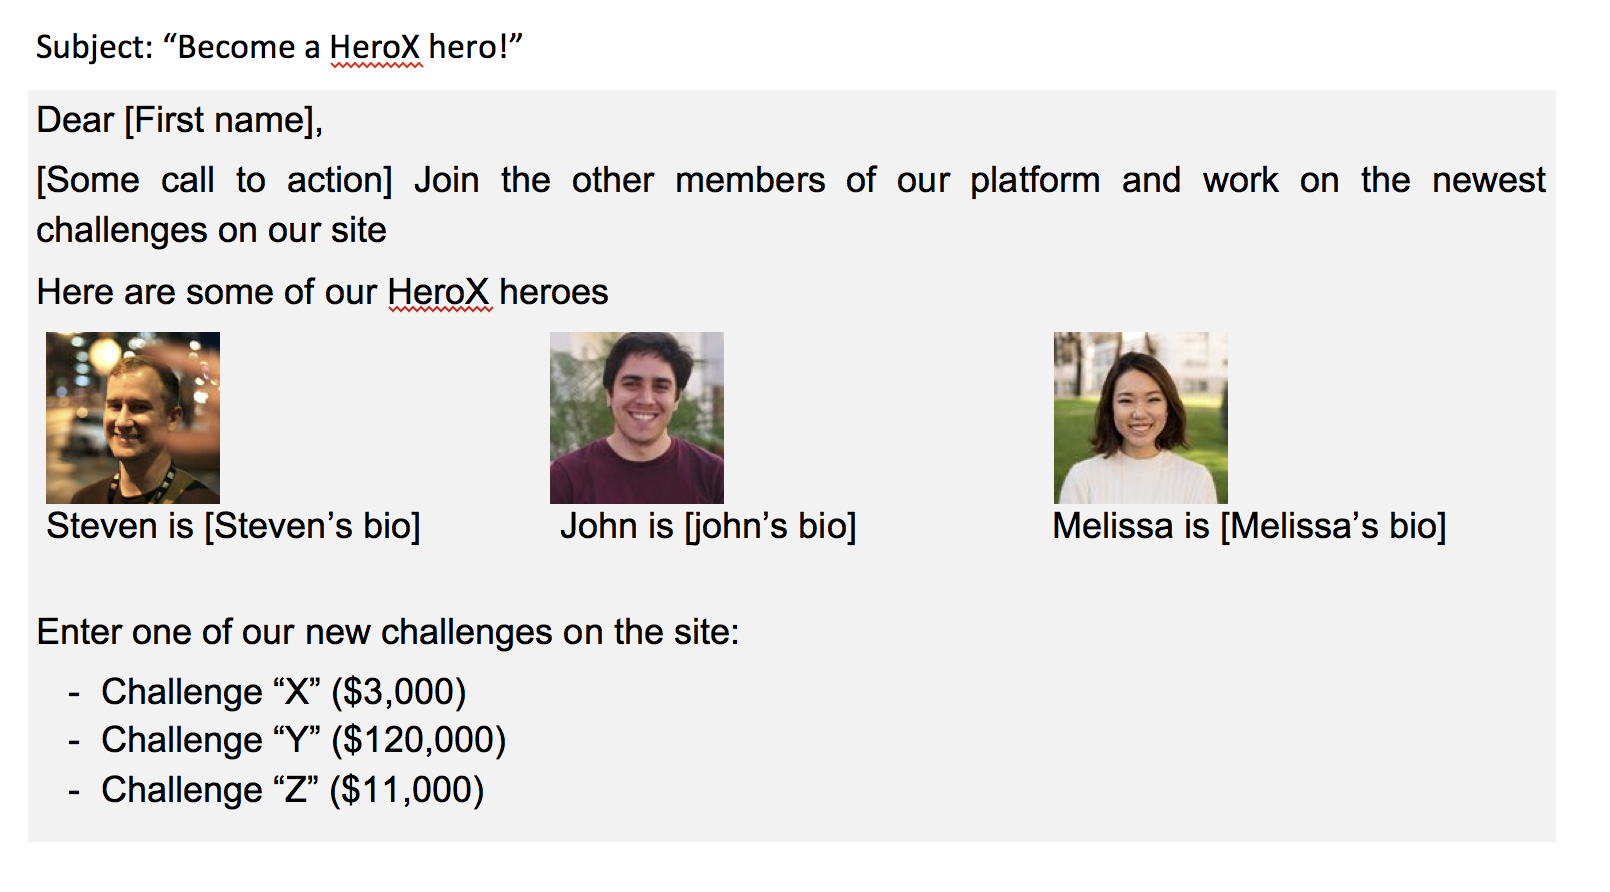
\includegraphics{solicit_gender_compo.png}
\caption{Solicitation email}
\end{figure}

\end{frame}

\begin{frame}{Treatment}

\begin{itemize}
\tightlist
\item
  Vary gender composition (look at ``Tokenism'')
\item
  Vary ``success'' composition
\end{itemize}

\begin{table}[ht]
\centering
\begin{tabular}{rll}
  \hline
 & Var1 & Var2 \\ 
  \hline
1 & 1 man role model & 3 women \\ 
  2 & 1 woman role model & 3 women \\ 
  3 & 1 man role model & 1 man 2 women \\ 
  4 & 1 woman role model & 1 man 2 women \\ 
  5 & 1 man role model & 2 men 1 woman \\ 
  6 & 1 woman role model & 2 men 1 woman \\ 
  7 & 1 man role model & 3 men \\ 
  8 & 1 woman role model & 3 men \\ 
   \hline
\end{tabular}
\caption{Treatment combinations} 
\end{table}

\end{frame}

\begin{frame}{Facebook/Twitter ads}

\begin{figure}
\centering
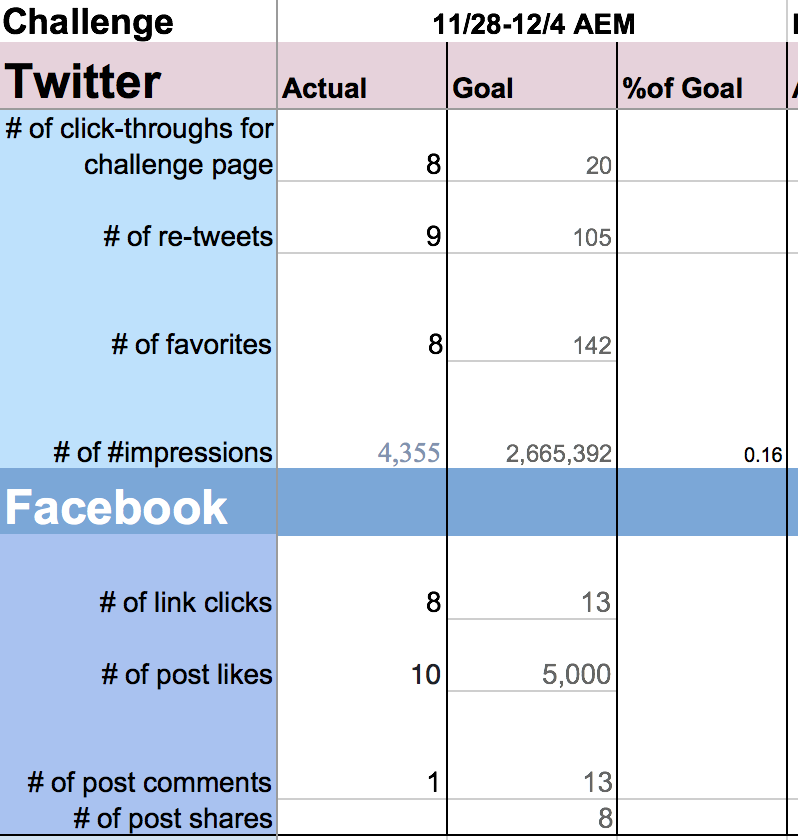
\includegraphics{ads.png}
\caption{Some statistics}
\end{figure}

\end{frame}

\begin{frame}{Validation of profiles}

Goal: comparable profiles

Use demographics + in the lab ratings of 20-30 profiles

\begin{itemize}
\tightlist
\item
  Physical attractiveness (based on user profile picture)
\item
  Role model (bio description + picture)
\item
  Skills
\end{itemize}

\end{frame}

\begin{frame}{Timing of the experiment}

\begin{enumerate}
\def\labelenumi{\arabic{enumi}.}
\tightlist
\item
  Preliminary survey (calibrate perceived gender composition)
\item
  Solicitation (email sent 1-2 times)
\item
  Ex-post survey (detect possible changes on perceived gender
  composition)
\end{enumerate}

\begin{itemize}
\tightlist
\item
  Outcome variables: participation, effort, team formation, etc.
\end{itemize}

\end{frame}

\begin{frame}{Example survey}

\begin{enumerate}
\def\labelenumi{\arabic{enumi}.}
\tightlist
\item
  Demographics (age, gender)
\item
  Motivations to participate in HeroX

  \begin{itemize}
  \tightlist
  \item
    {[}Cash prizes{]}
  \item
    {[}Learning{]}
  \item
    {[}CV/job opportunity{]}
  \item
    {[}Help society{]}
  \end{itemize}
\item
  What challenges do you like?

  \begin{itemize}
  \tightlist
  \item
    {[}STEM{]}
  \item
    {[}Social impact{]}
  \item
    {[}else{]}
  \end{itemize}
\item
  Estimate platform composition?

  \begin{itemize}
  \tightlist
  \item
    {[}Gender{]}
  \item
    {[}Age{]}
  \end{itemize}
\end{enumerate}

\end{frame}

\begin{frame}{Next steps}

\begin{enumerate}
\def\labelenumi{\arabic{enumi}.}
\tightlist
\item
  Identify profiles and ask for their consent (picture)
\item
  Recruit students to validate profiles
\item
  Send out preliminary survey
\item
  Ultimate solicitation message
\item
  Ads campaign with profiles
\item
  Examine results
\end{enumerate}

\end{frame}

\section{Collaboration incentives}\label{collaboration-incentives}

\begin{frame}{Basic idea}

\begin{enumerate}
\def\labelenumi{\arabic{enumi}.}
\tightlist
\item
  Male-female rich environment (how many teams?)
\item
  Splitting the pie rules (how many teams?)
\item
  Self-confidence
\end{enumerate}

\end{frame}

\begin{frame}{Technical requirements}

\begin{itemize}
\tightlist
\item
  Creating non-overlapping lists of potential teammates
\item
  Randomize composition of pool of potential teammates
\item
  Offer different incentives
\end{itemize}

\end{frame}

\begin{frame}{Example teaming}

\begin{figure}
\centering
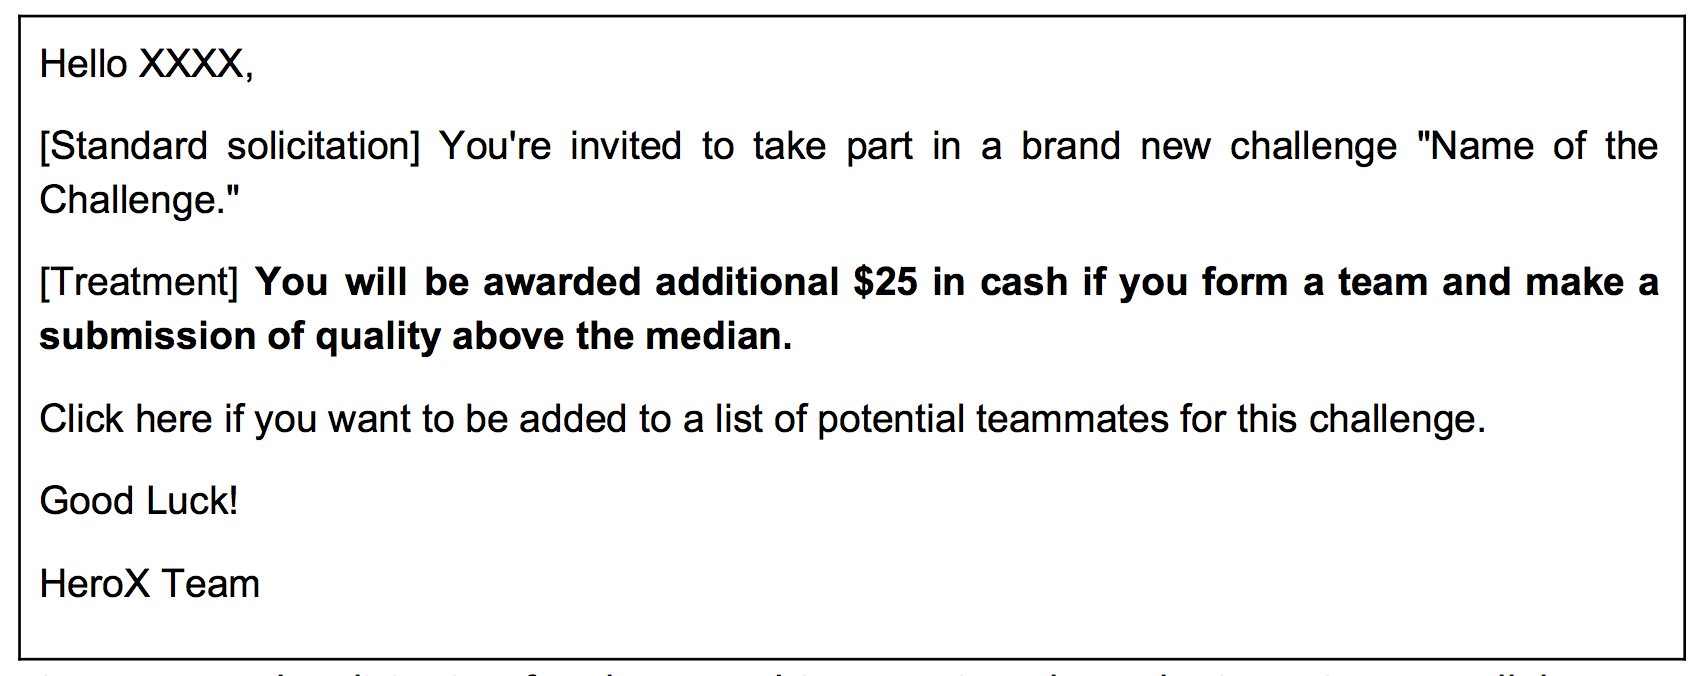
\includegraphics{solicit_teaming.png}
\caption{Teaming experiment}
\end{figure}

\end{frame}

\section{Thanks}\label{thanks}

\section{Demand estimation of the
challenges}\label{demand-estimation-of-the-challenges}

\begin{frame}[fragile]{Basic idea}

Launch \texttt{LinkedIn} campaign offering different pricing schemes

Examples:

\begin{enumerate}
\def\labelenumi{\arabic{enumi}.}
\tightlist
\item
  Fees vs no fees
\item
  Subsidizing prize money
\item
  Information treatment
\end{enumerate}

\end{frame}
